% rubber: setlist arguments --shell-escape
\documentclass{nle}

\newcommand{\makecite}[4]{\bibitem[\protect(\citename{#1 }#2)]{#3}#4}
\usepackage{graphicx,color,amssymb,times}
\usepackage[hidelinks]{hyperref}

\newcommand{\textoverline}[1]{$\overline{\mbox{#1}}$}

\title{Non-Native Text Analysis: A Survey}
\author[Sean Massung and ChengXiang Zhai]{SEAN MASSUNG and CHENGXIANG ZHAI \\
    Department of Computer Science \\
College of Engineering \\ University of Illinois at Urbana-Champaign \\
\texttt{\{massung1,czhai\}@illinois.edu}}
\received{25 November 2014; revised 12 March, 18 May, and 16 July 2015;\\
    accepted 20 July 2015}
\pagerange{\pageref{firstpage}--\pageref{lastpage}}
\pubyear{2015}

\newcommand{\todo}[1]{}
\renewcommand{\todo}[1]{{\color{red} TODO: {#1}}}

\begin{document}
\label{firstpage}
\maketitle

\begin{abstract}
Non-native speakers of English far outnumber native speakers; English is the
main language of books, newspapers, airports, air-traffic control, international
business, academic conferences, science, technology, diplomacy, sports,
international competitions, pop music, and advertising (British Council 2014).
Online education in the form of MOOCs (massive online open courses) is also
primarily in English---even teaching English. This creates enormous amounts of
text written by non-native speakers, which in turn generates a need for grammar
correction and analysis. Even aside from MOOCs, the number of English learners
in Asia alone is in the tens of millions.

In this paper, we provide a survey of the two main areas of existing work on
non-native text analysis, prefaced by an overview of common datasets used by
researchers, comparing their attributes and potential uses. Then, an
introduction to native language identification follows: determining the native
language of an author based on text in the second language. This section is
subdivided into various techniques and a shared task on this classification
problem. Next, we discuss non-native grammatical error correction---finding and
modifying text to fix errors or to make it sound more fluent. Again, we discuss
different methods before investigating a relevant shared task. Lastly, we end
with conclusions and potential future directions. While this survey primarily
focuses on detecting and correcting non-native \emph{English} text, many
approaches are general and can be used across any language pairing.
\end{abstract}

\section{Introduction}
\label{sec:introduction}

By the year 2020, the British Council (2014) estimates that there will be two
%By the year 2020,~\cite{british-council} estimates that there will be two
billion English language learners. Some learn in the classroom; some learn
online. Some may even learn through their phone or in an online class.
Regardless of the medium, computational tools to enhance this educational
experience will be valuable. Automatic scoring of essays---not only for grammar,
but also fluency---would contribute greatly to second-language learners'
understanding. User personalization for online services (including search
engines and social networks) would benefit from improved user profiling. More
relevant books or news articles could be recommended if the user's background
and competency of English were known.

Due to these many motivating examples, research in \emph{non-native text
analysis} has prospered. This field encompasses any textual task that deals with
words written in a language other than the writer's native tongue. We call the
native language L1 and the second, learned language L2. Throughout this survey,
we will usually assume that L2 is English, though most (but not all) techniques
discussed in this survey are general and could function with any pair of L1 and
L2.

Existing work in non-native text analysis is somewhat scattered, appearing in
workshops and shared tasks more frequently than standard proceedings. In this
survey, we provide a systematic overview of these scattered works to make it
easier for researchers to digest the state of the art in this emerging area.

\subsection{Scope}

The current work on non-native text analysis generally falls into two main
categories:

\begin{enumerate}
    \item \textbf{Native Language Identification} (NLI): classifying L1 based on
        text written in L2. Techniques can be categorized into
        \textbf{feature-based} (using a classifier) or \textbf{likelihood-based}
        (using a probabilistic model).
    \item \textbf{Non-native Grammatical Error Correction} (GEC): detecting and
        correcting grammatical errors in L2 text. Techniques can be categorized
        into \textbf{targeted} (correcting specific errors) or \textbf{general}
        (correcting all errors).
\end{enumerate}

Other subareas such as fluency scoring, non-native essay scoring, and text
simplification for non-native speakers also exist, but we focus this survey on
the two much larger areas explained above.

An excellent overview of grammatical error correction with a focus on non-native
learners is available~\cite{leacock-survey}. This short book is a concise
collection on the topic and consists of many recent advances since 2010. If the
reader wishes to delve into more detail in this subtopic, we suggest referencing
their work, whereas our paper is a broader outline and thus not able to go into
as much depth in one particular area.

Spelling correction described in Kukich (1992) is a potentially relevant
%Spelling correction described in\cite{1992-spelling} is a potentially relevant
task, though we choose to focus on the grammar correction aspect instead. This
is not to say that spelling features do not play a role in (\emph{e.g.}) NLI;
rather, the method of spelling correction is not relevant to non-native text
analysis. Correcting speech is also an important issue: besides the obvious
speech recognition challenges in computer science and electrical engineering,
speakers tend to voice their words much differently than when writing.
Therefore, we do not include any investigation into these works in this paper.

Shared tasks provide a common goal and dataset to a wide array of researchers.
This enables quick and accurate comparison of different methods, while
simultaneously increasing interest and producing exposure for the problem at
hand. Thus, we detail two relevant shared tasks in this survey that deal with
non-native writers of English. Author profiling, authorship attribution, and
plagiarism detection at PAN 2014~\cite{pan-2014} are also related, but we do not
focus on those here, instead considering them related works since there is no
specific component of non-native analysis.

Shared tasks have even started to evolve for L2s besides English. For example,
the Techniques for Educational Applications Workshop had a shared task on GEC
for Chinese as a foreign language~\cite{tea}.

\subsection{Organization}

We now review the structure of this paper. In each section, a figure briefly
summarizes the papers discussed and the methods used. If applicable, a
comparison of performance is also included. In this survey, we have a particular
preference for system papers as demonstrated by our sections on shared tasks. By
system papers, we mean research that immediately puts theory into practice,
giving real-world results which allow for better interpretation of effectiveness
by the reader.

First, in section~\ref{sec:datasets}, we introduce common datasets used in works
described throughout the rest of this survey. They should give some perspective
on the task at hand and create a mental baseline for the reader. We feel that it
is important to make note of these datasets here since any future work will most
likely be making use of these corpora.

In section~\ref{subsec:nli}, we start with an introduction to NLI, usually
formulated as a classification problem. Observed data is text written in L2
(where L2 means English: the second or foreign language), and a classifier
predicts the writers' L1 (the native language). Although this may be considered
a standard classification problem, the features chosen to target non-native
writer discrimination distinguish different approaches. These range from simple
unigram word counting to parse tree reranking descriptions. In future sections,
we will see how classifiers themselves may be adapted or configured to take
advantage of this specific domain.

Section~\ref{subsec:nli-shared} discusses the NLI Shared Task 2013 from the
Building Educational Applications (BEA) workshop. This shared task uses a corpus
detailed in section~\ref{sec:datasets}.

Section~\ref{subsec:grammar} discusses correcting grammatical errors, such as
articles and prepositions. These techniques are usually framed as classification
problems; a classifier determines if there is an error or not, and if so,
predicts what the best solution would be given a fixed set of candidates. Some
methods go beyond a simple classification setup and rely on more NLP-heavy
techniques such as language models and grammatical parse trees to find the
best corrected sentence.

Then, section~\ref{subsec:grammar-shared} covers the CoNLL 2013 and 2014 shared
task on grammatical error correction. This task also uses a corpus described in
section~\ref{sec:datasets}, and systems find and correct errors in text written
by non-native English speakers.

Finally, we end with a discussion and conclusions in
section~\ref{sec:conclusion}, reflecting on what issues may still be
unaddressed.

\section{Non-Native Corpora}
\label{sec:datasets}

\begin{table}[t]
\begin{center}
    \begin{tabular}{lrrccl}
    \hline
    \hline
    \textbf{Dataset} & \textbf{Docs} & \textbf{Len$_{avg}$} &
    \textbf{NLI} & \textbf{GEC} & \textbf{L1 Languages} \\
    \hline
    \hline
    CEEAUS & 1,008 & 128 & $\checkmark$ & & CHN, ENG, JPN (3) \\
    \hline
    CLEC & (1M & sent.) & & $\checkmark$ & CHN (1) \\
    \hline
    FCE & 1,244 & 200 & $\checkmark$ & $\checkmark$ & CAT, CHN, FRA, GER,\\
        & & & & & GRC, ITA, JPN, KOR,\\
        & & & & & NL, POL, PRT, RUS, SPA,\\
        & & & & & SWE, THA, TUR (16) \\
    \hline
    ICLE & 3,640 & 700 & $\checkmark$ & & BUL, CZE, FIN, FRA, \\
         & & & & & GER, ITA, NL, POL, \\
         & & & & & RUS, SPA, SWE (11) \\
    \hline
    ICLEv2 & 6,085 & 617 & $\checkmark$ & & BUL, CHN, CZE, FIN \\
           & & & & & FRA, GER, ITA, JPN, \\
         & & & & & NL, NOR, POL, RUS, SPA \\
         & & & & & SWE, TSW, TUR (16) \\
    \hline
    ICNALE & 5,600 & 129 & $\checkmark$ & $\checkmark$ & CHN, ENG, FIL, HKG, \\
           & & & & & IND, JPN, KOR, PAK, \\
           & & & & & SIN, THA, TWN (11) \\
    \hline
    NUCLE  & 1,397 & 863 & & $\checkmark$ & unknown \\
    \hline
    ETS & 12,100 & 348 & $\checkmark$ & $\checkmark$ & ARA, CHN, FRA, GER, \\
            & & & & &  IND, ITA, JPN, KOR, \\
            & & & & & SPA, TEL, TUR (11) \\
    \hline
    \hline
    \end{tabular}
\end{center}
    \caption{Comparison of non-native English datasets: corpus statistics, and
    whether they can be used for NLI or GEC\@. Web links to each dataset are
included in the text. Note that average document length may vary depending on
tokenization method.}
    \label{table:datasets}
\end{table}

All the work on non-native text analysis uses some kind of non-native text
corpus. In this section, we give an overview of the major datasets used in
existing work, which we will survey in the next few sections. As shown in
Table~\ref{table:datasets}, the sizes of these corpora vary from around one
thousand to twelve thousand documents with an average length of 128 to over 800
words. They cover a wide L2 range, geographically focused in Europe and Asia.
Abbreviations used in the table are ARA (Arabic), BUL (Bulgarian), CAT
(Catalan), CHN (Chinese), CZE (Czech), ENG (English), FIL (Filipino), FIN
(Finnish), FRA (French), GER (German), GRC (Greek), HKG (Hong Kong Cantonese),
IND (Indian languages), ITA (Italian), JPN (Japanese), KOR (Korean), NL (Dutch),
NOR (Norwegian), PAK (Urdu), POL (Polish), PRT (Portuguese), RUS (Russian), SIN
(Singapore languages), SPA (Spanish), SWE (Swedish), TEL (Telugu), THA (Thai),
TSW (Tswana), TUR (Turkish), and TWN (Taiwanese). We now give a detailed
description of each dataset.

ICLE~\cite{icle}, the International Corpus of Learner English, is an early
popular dataset used to investigate NLI\@. Its popularity is mostly due to the
fact that no other large NLI corpora existed at the time the ICLE was released.
It is a collection of essays on ``extremely varied'' topics written by
undergraduate students studying English. Additional metadata for each essay is
part of the ICLE---such as gender and age---though these features are rarely
used by researchers. Commonly, a five-language subset of Russian, Czech,
Bulgarian, French, and Spanish languages is used, popularized
by Koppel, Schler, and Zigdon (2005). These subsets caught on because the L1 distribution is
%by~\cite{koppel2005}. These subsets caught on because the L1 distribution is
quite unbalanced; the subsets have a more uniform distribution of native
languages. Thus, it is important to note if a subset of the ICLE is used so
accurate comparisons may be made. The corpus is publicly available, but requires
a license\footnote{\url{http://www.uclouvain.be/en-cecl-icle.html}}.

ICLEv2~\cite{iclev2} is an expanded version of the ICLE\@. There are no
major differences in the text files themselves (aside from the fact there are
more), since the ICLE is a subset. Version two additionally comes with a
\emph{concordancer}, a graphical interface that allows easy search and simple
exploratory analysis over the dataset. However, when running experiments
detailed in future sections of this paper, researchers tend to use the raw text
data from the corpus instead of any built-in software. The corpus is publicly
available, but requires a
license\footnote{\url{http://www.uclouvain.be/en-277586.html}}. The maintainers
of ICLEv2 are currently working towards releasing a third version.

CEEAUS~\cite{ceeaus} is the Corpus of English Essays written by Asian
University Students. Unlike the ICLE, the essays are restricted to two topics:
\emph{It is important for college students to have a part-time job} and
\emph{Smoking should be completely banned at all restaurants in the country}. A
common vocabulary for each prompt emerges due to this fact, perhaps allowing a
more meaningful word usage analysis to occur. Further restrictions attempt at
creating the most uniform testing conditions as possible: spell checking is
required, but dictionary use is prohibited; the writers have twenty to forty
minutes to complete their task. Aside from its small size, the main downside to
this corpus is that 77\% of the essays are from native Japanese speakers,
establishing a rather high classification baseline for NLI\@. A Web site exists
for the corpus, but it is no longer available to
download\footnote{\url{http://language.sakura.ne.jp/s/kaken_ceeaus.html}} since
it is a subset of ICNALE\@.

CLEC~\cite{clec} is the Chinese Learner English Corpus. It consists of one
million error-tagged sentences and is mainly used for grammatical error
correction. While there is no differentiation in L1, the dataset is segmented
into levels of English fluency. So while NLI classification is not possible, an
analysis on the skill level is feasible. Although free, the CLEC is only
available to members of the university that created
it\footnote{\url{http://langbank.engl.polyu.edu.hk/corpus/clec.html}}.

FCE, created by Yannakoudakis, Briscoe, and Medlock (2011), is the First
Certificate of English dataset---a corpus of essays written by students studying
English that took the Cambridge Assessment's ESOL (English as a second or other
language) exam. The dataset was compiled as a benchmark for automated essay
scoring systems, and contains about eighty types of correction annotations in
each essay. Like the ICLE, additional metadata is also included, such as grade,
age, and native language. There are ten different prompts, each with a varying
number of responses. This corpus may be downloaded freely
online\footnote{\url{http://ilexir.co.uk/applications/clc-fce-dataset/}}.

ICNALE~\cite{icnale}, the International Corpus Network of Asian Learners of
English, is an expanded version of CEEAUS\@. Like the ICLEv2, the previous
version is a subset of this one. Aside from adding more Asian L1 languages, the
language distribution of the dataset is much more balanced. Professional proof
readers corrected the part-time job essays, and their revised versions are also
included. This provides an opportunity to see how the non-native text is
translated into sounding more native---with this information it is possible to
do much more than NLI\@. The last segment of the ICNALE is a collection of 1,900
recorded speeches and their transcripts. After registering online, the corpus is
available\footnote{\url{http://language.sakura.ne.jp/icnale/download.html}} to
freely download.

NUCLE~\cite{nucle}, the National University of Singapore Corpus of Learner
English, is also a collection of essays on a wide variety of subjects. The
essays were written by students studying English at the Center for Language
Communication at NUS and annotated and corrected by English instructors.
Overall, nearly 47,000 errors were detected by the instructors with good rater
agreement. Findings on the corpus revealed that overall, errors in non-native
text are actually quite rare (at least in this corpus), on the order of around
four per one hundred words. Since this corpus was not intended for NLI, there is
no information about the L1 language of each essay. This is the dataset used by
the CoNLL 2013 shared task described in section~\ref{subsec:grammar-shared}, and
is available for download
online\footnote{\url{http://www.comp.nus.edu.sg/~nlp/corpora.html}}.

ETS~\cite{toef11} is a collection of essays from the Test of English as a
Foreign Language, a component of the Educational Testing Service. It is a
standardized test measuring English proficiency for students seeking to enroll
in college. There are 1,100 essays per L1, sampled from eight prompts. The
purpose of the corpus was to further enable work in NLI\@, and was used by the
BEA8 shared task described in section~\ref{subsec:nli-shared}. ETS is publicly
available, but requires a
license~\footnote{\url{https://catalog.ldc.upenn.edu/LDC2014T06}}.

From our comparison, we have two datasets that are subsets of another (CEEAUS
and ICLE). There is likely no reason to prefer CEEAUS over ICNALE or ICLE over
ICLEv2, since the newer versions are simply expanded. This leaves six main
datasets: CLEC, ETS, FEC, ICLEv2, ICNALE, and NUCLE\@. Of these six, CLEC, ETS,
FCE, ICNALE, and NUCLE, could be used for error analysis since they contain
annotations. All except CLEC and NUCLE can be used for native language
identification since the L1 information is part of the datasets.

As for content, all are essays written by university students, but only ICNALE
and ETS have the choice of essay topics strictly controlled---though the former
has two prompts and the latter has eight. ICNALE L1s are clearly focused in
Asia; NUCLE writers are most likely from Singapore, while FCE, ICLEv2, and ETS
L1s are more evenly distributed across the globe. Of course, CLEC consists of
all native Chinese authors.

Considering these differences, we need to think about the following questions
when interpreting results. What is the baseline accuracy? How difficult is it to
distinguish L1s? Does the number of documents (and document length) have any
bearing on an impression of the results?

Although not a standardized corpus, the website
Lang-8\footnote{\url{http://www.lang-8.com}} is also a popular location to
retrieve non-native English. This is a site where users write in a second
language and get corrections from native speakers. Corpora derived from this
site have been used for NLI~(\emph{e.g.} Brooke and Hirst (2011)) and
GEC~(\emph{e.g.} Tajiri, Komachi, and Matsumoto (2012)).

In the next sections, we systematically review the two areas of non-native text
analysis.

\section{Native Language Identification}
\label{sec:nli}

NLI is usually the first step in any second language error correction or author
profiling system. Identifying the native language of an anonymous text was first
popularized by Koppel et al. (2005). Brooke and Hirst (2012) do an extensive
survey of NLI feature efficacy, and develops a robust model that works well when
used across corpora. NLI tasks are most commonly evaluated solely on a small
learner corpus usually consisting of student essays (as shown in
section~\ref{sec:datasets}). It was previously thought that lexical features
would be biased or overfit towards essay topics, but a cross-corpus evaluation
showed that this was not the case~\cite{2012-robust-nli}.

For a more in-depth discussion of authorship attribution, we recommend the
reader consult two well-known surveys~\cite{aa-survey}~\cite{koppel-survey}.
Many techniques common to authorship attribution and author profiling are also
relevant to NLI.

As mentioned in section~\ref{sec:datasets}, the ICLE was an early popular
dataset to evaluate NLI tasks, especially using a subset of five European
languages partitioned by Koppel et al. (2005). A table has been created
(Table~\ref{table:nli-comp}) to portray the summary described in Brooke and
Hirst (2012). In addition to the results displayed in the table, Wong and Dras
also attempted to perform dimensionality reduction with LDA~\cite{lda} as
feature generation; however, this was not a successful method.

Techniques for NLI can be categorized into two methods: feature-based and
likelihood-based. Feature-based methods rely on informative features derived
from the text and are fed to standard machine learning algorithms (usually SVM
or MaxEnt). Likelihood-based methods learn a probabilistic model (usually a
grammar or language model) for each L1 and assign a label based on the maximum
likelihood model. We now move onto specific techniques applied in NLI.

\subsection{Techniques in Native Language Identification}
\label{subsec:nli}

The first feature-based method~\cite{tsur} found that incredibly simple
top two hundred frequent bigram character features fed to SVM led to $66\%$
accuracy on the five native languages. They claimed that word choice of
non-native speakers is influenced by the phonology of their native language (as
evidenced by the effectiveness of the character features). This approach is
compared to a unigram words baseline which achieved only $47\%$ accuracy. They
finally hypothesized that using a spoken-language corpus would achieve even
stronger results favoring character bigrams. Their reasoning was that much less
conscious effort is put into speaking than writing. For analyzing transcripts of
spoken words, the ICNALE corpus may be applicable, described in section 3.

NLI has also been approached through contrastive
analysis~\cite{wong2009contrastive}: the idea that errors in text are influenced
by the native language of the author. They investigated three error types as
features: subject-verb disagreement, noun-number disagreement, and determiner
misuse. These error types are then used as ``stylistic markers'' for NLI
features with an SVM classifier. To find these errors in text, they used an open
source grammar
checker\footnote{\url{http://queequeg.sourceforge.net/index-e.html}}, as opposed
to professionally edited text. Interestingly, ANOVA showed that the features had
a measurable effect, but after combining their contrastive features with
existing methods, they were not able to significantly increase the
classification accuracy from Koppel et al. (2005).

The previous authors~\cite{wong-rules} follow their work on contrastive
analysis, attempting to amend its shortcomings. Instead of error types, they use
two different features obtained from grammatical parse trees: horizontal slices
(production rules) and parse rerankings. They claim these are the first pure
syntactic features used in NLI\@. For the production rules, they immediately
applied information gain dimensionality reduction. The reranking features are
those contained in the Charniak parser\footnote{\url{http://cs.brown.edu/~ec/}}
and Stanford
Parser\footnote{\url{http://nlp.stanford.edu/software/lex-parser.shtml}} trained
on the Wall Street Journal. Unlike the previous two attempts, the authors found
MaxEnt to outperform SVM as the classifier. Additionally, five-fold cross
validation was performed (as opposed to ten-fold), which means the accuracies
cannot be precisely compared with previous work. In any event, they report a
final accuracy of $80\%$, which was the highest reported as of 2012.

\begin{table}[t]
  \begin{center}
    \begin{tabular}{llr}
        \hline
        \hline
        \textbf{Paper} & \textbf{Method} & \textbf{Accuracy} \\
        \hline
        (Tsur and Rappoport 2007) & character $n$-grams$^*$ & 66\% \\
        (Wong and Dras 2009) & syntactic errors$^*$ & 74\% \\
        (Wong and Dras 2011) & syntactic rules$^*$ & 80\% \\
        (Wong et al. 2012) & adaptor grammars$^{*+}$ & 76\% \\
        (Swanson and Charniak 2012) & tree substitution grammars$^{*+}$ & 78\%\\
        (Stolerman et al. 2013) & language family$^*$ & 80\%
        \\
        \hline
        \hline
    \end{tabular}
  \end{center}
    % can't have citations in captions for some reason...
    \caption{Summary of native language identification results listed in (Brooke
    and Hirst 2012) for the ICLE corpus; accuracies added to chart. $^*$
indicates feature-based methods and $^+$ indicates likelihood-based methods.}
    \label{table:nli-comp}
\end{table}

Wong, Dras, and Johnson (2012) explore the last author's---Mark Johnson's---adaptor
grammars~\cite{adaptor-grammars} to generate features. Simply, adaptor
grammars are a non-parametric extension to PCFGs (probabilistic context free
grammars). They can learn arbitrary-length word sequences (collocations); for
example, \emph{gradient descent} and \emph{cost function} were learned as
phrases in a machine learning topic. These adaptor grammars are used in two
ways: in the first, collocations are used as features in a MaxEnt classifier. In
the second, the grammar is trained on each class (representing native language).
At test time, the most probable grammar to have generated the text is selected.
For both tasks, the authors use five-fold cross validation on seven native
languages. In the feature-based classification, they achieved $76\%$; in the
language model-based classification, they achieved only $50\%$, a performance
similar to the unigram word baseline from Tsur and Rappoport (2007).

Swanson and Charniak (2012) made use of tree substitution grammars (TSGs)~\cite{tsgs}. TSGs are a tree-rewriting formalism that defines operations on
partial (parse) tree objects. For example, subtrees may be added or removed from
a base tree. Benefits of using this method are priors which prefer smaller
production rules and the ability to capture long-range dependencies. Various
induction methods are compared to generate features, and five-fold cross
validation on seven native languages is performed. All TSG features outperformed
the CFG baseline (at $73\%$). The highest TSG induction method was Bayesian
induction at $78\%$.

Massung, Zhai, and Hockenmaier (2013) also make use of grammatical parse tree features, but mainly
focus on their structural aspects as opposed to the syntactic category labels.
In one classification task, they found these features to work well in
determining the nationality of student essay writers from the CEEAUS dataset.
These structural parse tree features may be applicable in other tree-based
objects such as adaptor grammars, tree substitution grammars, and dependency
parses, but this has yet to be explored.

Lastly, Stolerman, Caliskan, and Greenstadt (2013) use language family as a feature for NLI\@. Specifically,
they took ICLEv2 documents classified with low confidence using unigram features
and reclassified them into one of the Germanic, Slavic, or Romance language
families. From there, the document was classified as an L1 using a subset of
training data only from the language family it was classified as. This method is
a type of hierarchical classification problem, and achieved about a $6\%$
increase over the baseline in NLI accuracy when using information gain feature
selection.

In summary, Table~\ref{table:nli-comp} lists the comparable accuracies from
experiments run on the ICLE/ICLEv2 subset of five European languages. In general
though, accuracies between 70\% to 80\% are standard for a wide variety of
techniques and corpora.

\subsection{Shared Task in Native Language Identification}
\label{subsec:nli-shared}

The 8th Building Educational Applications workshop held a shared task dedicated
to NLI~\cite{nli-shared}. Its goal was to increase visibility of
the problem and standardize results on a larger dataset: ETS\@. In total,
twenty-nine teams participated in the shared task.

There were three separate subtasks, differentiated by what data was allowed for
training:

\begin{itemize}
    \item \textbf{Closed Training}: use only the ETS corpus for training. All
        twenty-nine teams attempted this task.
    \item \textbf{Open Training I}: use any data \emph{except} the ETS corpus
        for training; the evaluation is still done on the ETS test set. Only
        three teams attempted this task.
    \item \textbf{Open Training II}: Use any data \emph{including} the ETS
        corpus. Only four teams attempted this task.
\end{itemize}

Overall results for the closed training were relatively close; the top thirteen
teams had between $80-83.6\%$ accuracy. The open training I subtask teams
performed much lower (probably as expected) at around 33, 38, and 57$\%$
accuracy. Finally, in the open training II subtask, none of the four teams were
able to beat the highest closed score. The most useful results for evaluating
models are probably those of the closed task, since all training data is
uniform, though it is interesting to see approaches employed to increase the
amount of training data. For example, in the open subtasks, other NLI datasets
were used such as ICLE, FCE, and ICNALE (all described in
section~\ref{sec:datasets}). Additionally, some teams crawled Lang-8, also
described in section 2.

\begin{figure}[t]
\begin{center}
\begin{minipage}[c]{.45\textwidth}
    \begin{center}
    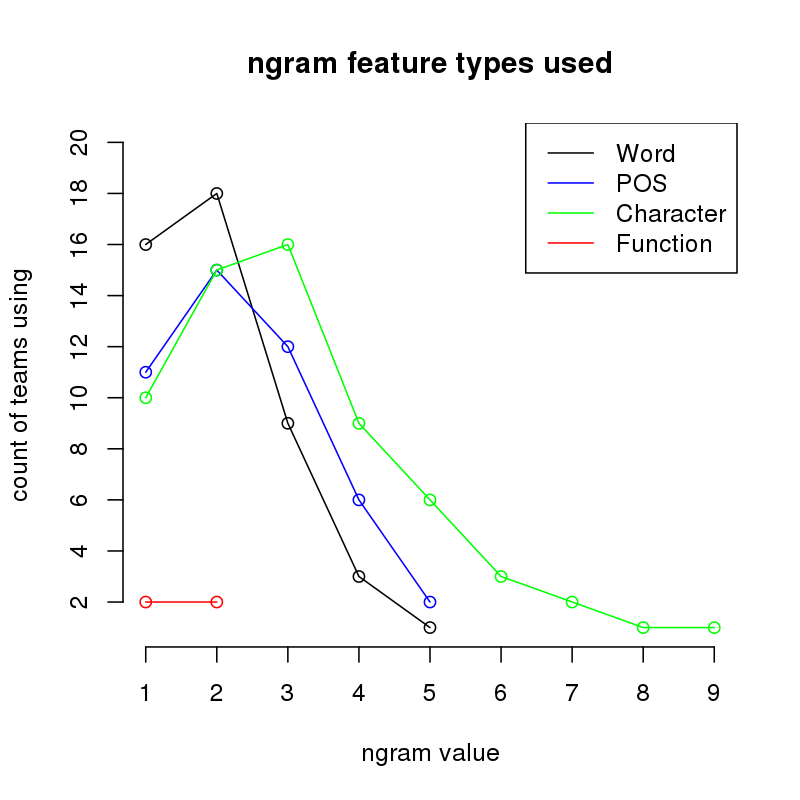
\includegraphics[width=2.3in]{ngram-comp}
    \end{center}
\end{minipage}
\hfill
\begin{minipage}[c]{.45\textwidth}
    \begin{center}
    \begin{tabular}{ll}
    \hline
    \hline
    \textbf{Classifier} & \textbf{Count} \\
    \hline
    SVM & 13 \\
    Ensemble & 4 \\
    MaxEnt & 3 \\
    DFA & 1 \\
    String kernel & 1 \\
    PPM & 1 \\
    $k$-NN & 1 \\
    \hline
    \hline
    \end{tabular}
    \end{center}
\end{minipage}
\caption{Number of teams using particular $n$-gram features (left) and number of
teams using a particular machine learning algorithm (right). DFA and PPM refer
to discriminant function analysis and prediction by partial matching.}
\label{fig:ngram-comp}
\end{center}
\end{figure}


The most common features used were $n$-grams of lexical tokens such as words or
part-of-speech tags; Figure~\ref{fig:ngram-comp} compares the $n$-grams used by
all teams. Aside from these, some less common features were grammatical:
dependency parses, TSGs~\cite{tsgs}, parse tree rules, and adaptor grammars~\cite{adaptor-grammars} were used. Spelling error features were also
captured by three of the teams. These features are all described in work in
section~\ref{subsec:nli}. Below, we outline a few of the more unique feature
representations.

Skipgrams~\cite{skipgrams} were an $n$-gram variant feature used by several
teams. Instead of considering an $n$-gram to consist of $n$ adjacent words in
the text, a $k$-skip $n$-gram allows up to $k$ words total to be skipped in a
sequence of tokens. Given the sentence ``\emph{They all studied statistics
Monday evening}'', normal 3-grams would be $\{$\emph{They all studied, all
studied statistics, studied statistics Monday, statistics Monday evening}$\}$. A
few possible 2-skip 3-grams are $\{$\emph{They all studied, They studied
statistics, They statistics Monday}$\}$. This attempts to capture important
phrases without regard to interspersed function words. Using skipgrams was shown
to reduce perplexity on a testing set, as well as offer a viable alternative to
increasing the corpus size (which is usually not feasible). Since most NLI
datasets we have examined are relatively small, using skipgrams could help
improve language modeling. While interesting, none of the teams in the top third
used skipgrams in their systems.

For one feature type, the system by LIMSI used a form of machine translation
called ``back translations''~\cite{nli-mt}. A back translation attempts to
capture a writer's lexical preference for a word sense. For example, LIMSI found
that the English word sense for \emph{awkward} is more likely to be written as
\emph{clumsy} by native Spanish speakers. These word preferences were used as
features in addition to other features: word $n$-grams, spelling mistakes, and
grammatical mistakes. Adding the back translation features slightly increased
the task's overall classification accuracy, but the team still performed poorly
overall.

The CMU-Haifa team used a ratio of passive to active verbs in their
system~\cite{nli-passives}. They operated under the common assumption that
English uses passive voice more frequently than other languages, and the amount
of passive use may vary based on the writer's L1. Recall that passive voice is a
literary technique that shifts attention away from the one performing an action.
``\emph{The passive voice is often used}'' is a sentence in the passive voice;
``\emph{English speakers often use the passive voice}'' is a sentence in the
active voice. The passive voice is characterized by the verb \emph{to be} and
the past participle of the verb. In the previous sentences, we have \emph{is
used} and \emph{use} conjugated differently. Using the passive ratio feature
exclusively yielded a $12\%$ accuracy on a $9\%$ baseline. In combination with
four other main features, the accuracy was not significantly improved. However,
further investigation could be warranted to examine the usefulness of such
stylistic composition features.

SVM was by far the most prevalent classifier employed by the teams, as displayed
in Figure~\ref{fig:ngram-comp}. Below, we outline some of the more uncommon
classifiers.

Discriminant function analysis (DFA) from statistics was used
for increased interpretability over other methods~\cite{nli-dfa}. Using this model, they were
able to find correlations between different L1s. For instance, Japanese and
Korean L1s were highly correlated in their underuse of the words $\{$\emph{all,
any, but, different, or, person, this, your}$\}$. Unsurprisingly, languages of
similar origin were also correlated---the Romance languages were often
misclassified as one another due to increased correlation of $n$-gram tokens.
Unfortunately, this team performed poorly overall.

Originally designed to operate on DNA sequences, the string kernel model~\cite{2013-stringkernel} is given a stream of characters. Specifically,
a kernel based on local rank distance is used for native language
identification. The simplest string kernel function $f(w_1,w_2)$ counts the
number of substrings of a particular length that $w_1$ and $w_2$ share. It is
also quite intuitive to introduce a normalized version that is not biased by
long words. Local rank distance is then an extension that counts the sets of
\emph{similar} $n$-grams between $w_1,w_2$. In their NLI context, each word was
actually a character $n$-gram. This method has the advantage that no syntactic
information is needed; no parsing or even sentence or word segmentation is
required. In training, they found that $n\in[5,8]$ gave the best results,
allowing them to take third place overall in the closed task.

Similar to the string kernels previously, Bobicev (2013) uses a method which
requires very little text processing: prediction by partial matching (PPM), a
statistical compression method. The output of PPM is a language model which can
be used to find the highest likelihood L1 given some unknown text. Both words
and characters were used as tokens, though character features performed much
worse than words, obtaining a precision of $37\%$ (compared to $70\%$ from the
word tokens) on the 9,900-document training set. This performance placed the PPM
features in the bottom third of contestants.

\begin{table}[t]
\begin{center}
    \begin{tabular}{llr}
        \hline
        \hline
        \textbf{Paper} & \textbf{Method} & \textbf{Accuracy} \\
        \hline
        \hline
        (Jarvis et al. 2013) & SVM on lexemes, lemmas, POS & 83.6\% \\
        \hline
        (Bykh and Meurers 2014) & ensemble many lexical/syntactic & 84.8\% \\
        \hline
        (Ionescu et al. 2014) & character string kernels & 85.3\% \\
        \hline
        \hline
    \end{tabular}
    \caption{Increasing state-of-the-art NLI accuracy results for the ETS
    dataset.}
    \label{table:ets}
\end{center}
\end{table}

In conclusion, most methods used by teams in the NLI shared tasks were very
standard (\emph{e.g.} $n$-grams of words with SVM). In fact, the winning
team~\cite{jarvis} with 83.6\% accuracy used SVM with unigram to trigrams of
log-entropy weighted lexemes, lemmas, and POS tags. A small number of teams
investigated some unique text representations and classification techniques.
Given options between feature-based and likelihood-based strategies, most teams
focused on features. While not always successful, these new methods can be
further explored and analyzed in future work. Table~\ref{table:ets} summarizes
the results discussed on the ETS dataset. After the contest ended, others
have surpassed the highest-scoring Jarvis et al.\ team.

First, Bykh and Meurers (2014) considered an ensemble of various
features, consisting of context-free grammar rules and forty $n$-gram
representations of words, POS tags, and lemmas for $n\in[1,10]$. They found
training a separate classifier for each feature type gave definite advantages
over concatenating feature vectors.

Second, Ionescu, Popescu, and Cahill (2014) improved over Bykh and Meurers
(2014) by using only
character-based features. However, the way that the character features are used
is advanced. They combined various string kernels with two learning methods,
kernel ridge regression and kernel discriminant analysis. We suggest that the
reader consult their paper for a more in-depth description of these tools. Their
best results were when string lengths were in the range $[5,8]$. Seven of their
kernel and learning combinations outperformed the first place shared task
team~\cite{jarvis}, and their best two combinations best the Bykh and Meurers
score. Their highest-scoring setup was kernel discriminant analysis on a
weighted combination of a presence bits kernel (dot product of occurring
characters) and the intersection string kernel.

\section{Non-Native Grammar Correction}
\label{sec:grammar}

We now transition from native language identification to non-native grammar
correction. While the former is often tackled as a one-step task, the latter
usually relies on classification as a component, but also consists of other
parts that are able to capture a deeper syntactic meaning (such as dependencies
or language modeling). Correcting machine translated text is a related issue,
but we do not discuss it here; instead, please see Corston-Oliver, Gamon, and
Brockett (2001) or Gamon, Aue, and Smets (2005).

In the section~\ref{subsec:grammar}, we discus some key papers that display a
wide variety of techniques. We also briefly touch on training data issues as
well as evaluation of corrected text. Section~\ref{subsec:grammar-shared}
outlines the CoNLL shared task in grammatical error correction for 2013 and
2014.

\subsection{Techniques in Non-Native Grammar Correction}
\label{subsec:grammar}

Some grammar correction methods are targeted towards a very specific subset of
errors, often categorized by the corpus; others attempt to solve more general
errors concerning word sense or collocations. Evaluation for grammar correction
is much more varied and unstandardized in comparison to the configurations from
NLI seen in the previous section. Which non-native corpus is used also dictates
the types of errors that can be corrected. Table~\ref{table:gec} compares the
different methods discussed in this section and categorizes them as either
targeted or general approaches.

Lee and Seneff (2006) train a trigram language model on a lattice of alternatives,
where ``alternatives'' are prepositions, articles, and auxiliaries that may or
may not occur between words in the original text. For example, the sentence
\emph{I want flight Monday} can be corrected by inserting two tokens as such:
\emph{I want a flight on Monday}. Their algorithm first strips all such
alternatives from the original sentence. So far, this is not much different from
the article and preposition corrections. However, they additionally change each
remaining word in the input sentence to be a set of related words to the base
form: $want~\rightarrow~\{want, wants, wanted, wanting\}$. Their language model
then outputs the $k$-best candidates. Next, these candidates are given to a PCFG
and reranked. The final output is the top-ranked sentence from the PCFG\@.
Across all experiments, they found that reranking the language model candidates
significantly increased the $F$ measure.

\begin{table}[t]
    \begin{center}
    \begin{tabular}{lll}
        \hline
        \hline
        \textbf{Paper} & \textbf{Method} & \textbf{Target} \\
        \hline
        (Lee and Seneff 2006) & LM with PCFG scoring$^*$ & articles, prepositions,\\
                              & & and word forms \\
        (Gamon 2010) & classifier ensemble$^*$ & articles and prepositions \\
        (West et al. 2011) & bilingual random walk$^+$ & word sense \\
        (Dahlmeier and Ng 2011a) & machine translation$^+$ & collocation errors \\
        (Dahlmeier and Ng 2011b) & structure optimization$^*$ & articles/prepositions \\
        (Madnani and Tetreault 2012) & machine translation$^+$ & common errors\\
        \hline
        \hline
    \end{tabular}
    \caption{Comparison of grammatical error correction strategies. $^*$
    indicates targeted approaches and $^+$ indicates general approaches.}
    \label{table:gec}
    \end{center}
\end{table}

West, Park, and Levy (2011) use bilingual random walks between L1 and L2 word senses. For
example, on one side of a bipartite graph are L1 words. There are connections
from a word $w\in$ L1 to a word $w'\in$ L2 if a $w$ could be translated into
$w'$. $w$ could be the English word \emph{head}, and be translated into a
physical head, head of an organization, or the verb \emph{to head}. This model
was used to correct non-native sounding phrases such as \emph{entire stranger} to
the more natural \emph{complete stranger}. This bipartite graph was combined with
a language model to correct non-native sentences. In these experiments, the
native language was Korean. Evaluation was performed with Amazon Mechanical
Turk~\footnote{\url{https://www.mturk.com/mturk/welcome}} where workers chose
between the corrected sentence and the original sentence. Results were not
strongly positive, since sometimes the corrected errors changed the meaning of
the sentence or made it ungrammatical. In future work the authors suggest using
a richer probabilistic model such as a PCFG.

Dahlmeier and Ng (2011a) use the NUCLE corpus to find and correct collocation errors via
machine translation. Here, a collocation is a phrase commonly used by native
speakers. The authors propose that when a writer mentally translates from L1 to
L2, some unnatural phrases result due to word choice. They give an example,
``\emph{I like to look movies}'' that might be written by a native Chinese
speaker since \emph{watch} and \emph{look} are very similar in the L1. It would
be possible to correct this to the more grammatical ``\emph{I like to look at
movies}'', but it still does not sound natural. Instead, \emph{look} is replaced
by \emph{watch}, resulting in the more fluent collocation \emph{watch movies}.
For their experiments, they assume the unnatural collocations have already been
identified; this mimics a system where a user may ask for improvement
suggestions for a snippet of writing. They train a statistical machine
translation model on a parallel Chinese-English corpus to correct collocation
errors in the NUCLE corpus. A log-linear model was used to score the candidate
phrases which allows additional spelling, homophone, and synonym features to be
incorporated. They evaluated their method as a retrieval task, where they
returned the top $k$ suggestions to fix each collocation error. Two
native-English speakers judged results from five hundred corrections with good
rater agreement. Finally, they performed an analysis of errors and found that
the main reason top-ranked phrases were not correct was due to out-of-vocabulary
words.

Dahlmeier and Ng (2011b) introduce an alternating structure optimization (ASO)
approach to GEC\@. In short, ASO is able to leverage a
common structure between multiple related problems; see Ando and Zhang (2005) for a more
detailed description. In this case, the related problems are selection (find
features from native text) and correction (fix the errors in non-native text).
Targets were article and preposition errors, again using the NUCLE corpus.
It was shown that ASO significantly outperformed a simple linear classifier as
well as two unnamed commercial grammar checkers. Features included
part-of-speech tags, hypernyms from WordNet, named entities, and shallow parsing
tags.

Gamon (2010) combined a language model and classifier into a
``meta-classifier'' that detected errors in both article and preposition use.
Additionally, they investigated how much more training data is needed for the
individual methods to approach the accuracy of the meta-classifier. Features for
the classifier were a window of six tokens to the right and left of errors, POS
tags, and lexical head features. The classifier was actually split into two
steps: first, determine the likely presence of a preposition or article. Then,
determine \emph{which} article or preposition should be chosen. The language
model is trained on LDC's \emph{Gigaword} corpus and log-likelihood was
used (normalized by sentence length). The meta-classifier uses features
generated from the two primary models such as ratio of likelihood scores from
the language model and classifier decisions. As expected, the meta-classifier
outperformed the two simpler models. Prepositions were harder to classify than
articles and they required more training data to reach a specific level of
accuracy. Future work would be including more primary models to feed features
into the meta-classifier.

Madnani, Tetreault, and Chodorow (2012) applied ``round-trip'' machine translation to correct generic
errors in L2 text. A round-trip translation used the Google Translate
API\footnote{\url{http://research.google.com/university/translate/}} to
translate the candidate text from L2 to eight different languages and back again
to L2. Since it is not guaranteed that the translations will preserve the
meaning of the sentence, they assert that using a language model to select the
most fluent choice is not acceptable. Instead, they combined alignments between
the source and each round trip translation to create the final answer. This
method had a better likelihood of maintaining the sentence's original meaning.
In order to evaluate their system, they had human graders check whether the
fixes were fluent as well as retaining the original meaning.

The next two papers we discuss consider alternatives to standard acquisition of
training data for GEC\@. Usually, a dataset with annotated areas as described
from section~\ref{sec:datasets} is used, but these papers create or acquire
their own non-native errors.

Instead of training directly on non-native text, Rozovskaya and Roth (2010) took
native text and intentionally inserted article errors. In order to create a
realistic error distribution, they generated the article errors with the same
observed distribution as the non-native corpora. Advantages to training data
generation in this style are avoiding expensive data annotation, circumventing
small corpus sizes, and tailoring the classifier to a particular language. Most
of all, their method was shown to be superior to only training a classifier on
purely native data. One final note they make is that previous baselines used in
the literature are not always appropriate; baselines mentioned before are simply
the majority class. While this is acceptable for a selection task, this ignores
the actual error rate in the data. Usually, the error rate is much lower (shown
to be about 10\% in their experiments) than the majority class. Therefore, they
argue, a more fair comparison would be the \emph{error reduction}, and this is
indeed the measure they use to report their results. They reduced the error
detection in native Chinese, Czech, and Russian text by 10\%, 5\%, and 11\%
respectively.

The next authors~\cite{wiki-rev} obtained their grammatical errors from Wikipedia revisions. They
filtered the article revisions dataset looking for single-word changes that
corresponded to correcting article and preposition errors. Using this method,
they obtained over one million corrections. They compared their mined corpus
with standard error correction corpora as well as artificially-inserted errors
like Rozovskaya and Roth's approach. They found that the larger ``somewhat
clean'' Wikipedia edits were much better in increasing the $F_1$ of the grammar
corrector as opposed to other common datasets, including a smaller ``more
clean'' version of their Wikipedia data. Furthermore, they found that artificial
error insertion methods trained on their Wikipedia revisions data increased
system accuracy compared to training on smaller corpora, and even generalized
across datasets.

In sharp contrast to NLI evaluation, Chodorow, Dickinson, Israel, and Tetreault
(2012) describe many issues
regarding evaluation for grammatical error correction, with a focus on
non-native sentences. This is a valuable paper for those engaging in any GEC
task. Their main issue is the ``three-way contingency'' between the original
sentence, the human correction, and the system output (let alone the evaluation
scripts themselves). Mentioned later~\cite{2013-joint}, this report also
emphasizes the significance of the relatively low error rates in non-native
sentences---this phenomenon suggests using more interpretable measures such as
true and false positives and negatives. Furthermore, how is the severity of an
error taken into account? For example, most native English speakers often misuse
\emph{who} and \emph{whom}. Their conclusion from these observations is to
develop a robust evaluation system based on raw error type counts. This allows
bias and error skewness to be perceived by the reader while simultaneously
permitting the reader or other evaluator to map the raw error data into another
form such as precision, accuracy, prevalence, or bias.

\subsection{Shared Task in Non-Native Grammar Correction}
\label{subsec:grammar-shared}

We continue our discussion on GEC with the introduction of the
CoNLL-2013 shared task~\cite{2013-task-all} and the CoNLL-2014 shared task~\cite{2014-task-all}. The training data was the NUCLE
corpus, containing annotations categorized by five error types in 2013 along
with the corrected text. In 2014, there were a total of twenty-eight error
types, many of which were subcategories of the 2013 types. Some systems first
classified potential errors by error type and then corrected errors while others
made no such distinction. Additionally, the teams received preprocessed input:
sentence segmentation, word tokenization, and part-of-speech tagging were all
performed.

In all, there were 1,397 essays consisting of 57,151 total sentences. Article
and determiner errors were most prevalent. Testing data was considerably smaller
with only fifty essays each year. Teams were also allowed to use any external
resources that were non-proprietary and publicly available.
Table~\ref{table:grammar-comp} shows the methods of the top teams from both
years. The five error types from 2013 are listed below:

\begin{itemize}
    \item \textbf{Article or determiner}: ``\emph{In late nineteenth century,
        there was a severe air crash happening at Miami international
        airport.}'' Correction: replace \emph{late} with \emph{the late}.
    \item \textbf{Preposition}: ``\emph{Also tracking people is very dangerous
        if it has been controlled by bad men in a not good purpose.} Correction:
        replace \emph{in} with \emph{for}.
    \item \textbf{Noun number}: ``\emph{I think such powerful device shall not
        be made easily available.}'' Correction: replace \emph{device} with
        \emph{devices}.
    \item \textbf{Verb form}: ``\emph{However, it is an achievement as it is an
        indication that our society is progressed well and people are living in
        better conditions.}'' Correction: replace \emph{progressed} with
        \emph{progressing}.
    \item \textbf{Subject-verb agreement}: ``\emph{People still prefers to bear
        the risk and allow their pets to have maximum freedom.}'' Correction:
        replace \emph{prefers} with \emph{prefer}.
\end{itemize}

While the contest setup and evaluation does not completely mimic real-life
scenarios, it does provide useful information for those interested in GEC\@.
Since the errors are categorized into groups, it is possible to perform an error
analysis on the results.

As mentioned previously, even performing the evaluation is not a trivial task;
suggested corrections---while completely valid---may not actually match the
``official'' corrections. To mitigate these issues, the contest organizers
permitted the contestants to submit their own gold standard corrections if they
disagreed with the provided answers. Of course, the corrections were reviewed.
It is also worth noting that the training and test data contained errors other
than those in the five categories, but these additional errors were not taken
into consideration in the final scoring.

\begin{table}[t]
  \begin{center}
      \begin{tabular}{llll}
       \hline
       \hline
       \textbf{Team} & $P$ & $R$ & $F_{\{1,0.5\}}$\\
       \hline
       \hline
       UIUC (Rozovskaya et al. 2013)& 46.45 & 23.49 & 31.20$_{F1}$ \\
       \hspace{.1in}averaged perceptron and Na\"ive Bayes & & &\\
       \hline
       NTHU (Kao et al. 2013)& 23.80 & 26.35 & 25.01$_{F1}$ \\
       \hspace{.1in}$n$-gram and dependency language model & & & \\
       \hline
       HIT (Xiang et al. 2013)& 35.65 & 16.56 & 22.61$_{F1}$ \\
       \hspace{.1in}MaxEnt and rules & & & \\
       \hline
       \hline
       CUUI (Rozovskaya et al. 2014) & 52.4 & 29.89 & 45.57$_{F0.5}$\\
       \hspace{.1in} error interaction via joint inference & & & \\
       \hline
       CAMB (Felice et al. 2014) & 46.70 & 34.30 & 43.55$_{F0.5}$\\
       \hspace{.1in} pipeline and error type filtering & & & \\
       \hline
       \hline
      \end{tabular}
  \end{center}
      % can't have citations in captions for some reason...
      \caption{Top teams from the CoNLL-2013 and CoNLL-2014 GEC shared task.}
      \label{table:grammar-comp}
\end{table}

The 2013 third-place team~\cite{2013-task-hit} from Harbin Institute of
Technology (HIT), split their system into two parts: a machine learning module
(article \emph{vs} determiner, prepositions, and noun errors) and a rule-based
module (verb form and subject-verb agreement). As indicated in
Table~\ref{table:grammar-comp}, the classifier used was a Maximum Entropy classifier
with additional feature selection via genetic algorithms and confidence tuning
based on the maximum entropy score. The rules were first preprocessed with the
frequent pattern mining algorithm FP-growth to find common incorrect phrases.
These common phrases were then removed from the candidate set to be corrected. A
list of these common phrases was provided and may prove useful for future work.
In their results, they found that their models were very sensitive to the
parameters and that the confidence tuning had the largest positive effect in
their pipeline.

National Tsing Hua University (NTHU)~\cite{2013-task-nthu} finished in
second place in 2013 with a system that was very similar to theirs from the
previous year. In the CoNLL-2013 shared task, subject-verb agreement was not a
labeled error type so the NTHU system ignored these errors. In the seemingly
current trend, a module was created for each error type, though their modules
were more similar to each other than the previous systems. Each module used a
moving window of words up to length five---five here because they leverage the
Google 5-gram corpus as well as their previous tool
Linggle\footnote{\url{http://linggle.com}}. Linggle is a linguistic search
engine in which the user can specify wildcards for nouns, verbs, and
adjectives~\cite{linggle}. Results were returned with those wildcards filled in
ordered by increasing likelihood in the dataset. These likelihoods were used to
score candidates generated by their system in each module. Their candidate
voting system was created using a backoff model of lower-order $n$-grams. Verb
form errors were really the only significantly different module by including
pointwise mutual information.

The University of Illinois at Urbana-Champaign (UIUC)~\cite{2013-task-uiuc}
had the best-performing system in 2013. They made use of previous work for
article errors (with averaged perceptron) and preposition errors (with Na\"ive
Bayes). The remaining three error classes were dealt with Na\"ive Bayes with
priors trained on the same Google corpus that NTHU used. Although the CoNLL
corpus already contained part-of-speech tags, they reparsed the dataset with
their own tools in addition to running a shallow parser for feature generation.
There was no pipeline in the system, meaning that corrections of each model were
pooled together to create the final output sentence. In their error analysis,
they found that an incorrect verb form can cause parsers to break, which greatly
hindered rule-based methods. Since the errors were so sparse, they hypothesize,
less complicated machine learning algorithms would be more robust to the large
amount of noise. This analysis provided much insight and would be useful for
future work.

After the contest ended, UIUC~\cite{2013-joint} returned to the
CoNLL-2013 shared tasks with a joint learning and inference approach. Based on
their observations from the shared task, they reasoned that individual (read:
\emph{independent}) classifiers per word do not capture interactions between
errors and word choice. They accomplish this by combining individual classifiers
using integer linear programming---a model which is able to jointly learn the
error occurrences. They thus increased the $F_1$ score on the CoNLL-2013 data to
$42\%$, significantly higher than their first place score. They do note though,
that $F_1$ may not be an appropriate measure; it is indeed more intuitive to
measure the increase in correctness of the original data since it is quite
likely that the grammar correction systems actually introduce errors themselves.

Cambridge University~\cite{2014-hybrid}  was the second-best team in 2014.
Without additional error suggestions for evaluation, they were in first place.
They used a pipeline-based system which first ran rule-based corrections with a
tool designed for English learners at their school. A language model selected
the best candidate sentences from the rule-based edits. Then, those candidates
were sent to a statistical machine translation system trained on parallel
English data, which included NUCLE and FCE (see section 2). Then, a large 5-gram
language model from Microsoft was used to select candidates for the final stage.
This is the main novelty of their system: with these final candidates they
filter the error correction types to ignore unnecessary corrections. Their
classifier was able to label almost $70\%$ of error types correctly on
development data. They filtered out the labeled types that had zero precision,
which consisted of reordering errors, run-ons, comma splices, and acronyms.
Although the filtering did increase their $F_{0.5}$ score, the difference was not
statistically significant. This is an example of how evaluation metrics play an
integral part in system design.

Columbia University and the University of Illinois at
Urbana-Champaign~\cite{2014-cuui} was the top team in 2014. They improved upon their system from
the previous year, and also included their joint inference work
\cite{2013-joint}. The last addition was the inclusion of new classifiers for
the different error types; in total they had sixteen classifiers targeting the
twenty-eight error types. The classifier learning algorithm for each error type
was one of Na\"ive Bayes, Na\"ive Bayes with priors, and averaged perceptron.

In conclusion, we saw a variety of techniques for correcting grammatical errors,
which can be categorized into targeted \emph{vs} general strategies. Targeted
strategies focus on errors of only specific types (such as the shared task)
which general correctors try to improve the overall fluency of the L2 text.

\section{Conclusions}
\label{sec:conclusion}

We realize that support for dealing with non-native text is becoming
increasingly important; many applications benefit from automatic author
profiling and grammatical error correction. We call this collection of
challenges and tasks \emph{non-native text analysis}. This survey detailed
common datasets and covered the two main applications in non-native text
analysis: native language identification and grammatical error correction.

In section~\ref{sec:datasets}, we saw the main corpora used by researchers for
NLI and GEC. Compared to other text datasets, these are relatively small and
only consist of essays written by students. A larger corpus would be beneficial,
as would a corpus of text other than essays such as blogs, social media, or
research papers. Finally, the availability of such datasets are directly
proportional to the amount of impact they may have; freely available corpora are
much more likely to be used than their proprietary counterparts.

Section~\ref{sec:nli} detailed NLI as a classification problem. We also saw how
a shared task was able to elicit many quality works from the community in an
organized fashion. We subdivided NLI approaches into two techniques: feature-
and likelihood-based. Much more effort has been put into feature-based methods
using standard machine learning algorithms. Instead of classifiers and
probabilistic models, is it possible to use other text mining algorithms? For
example, can clustering methods be optimized for use with NLI? What is the
significance of outliers and dense subclusters? How do collaborative filtering
systems change when additional information about learning styles of users are
known?

Grammatical error correction was discussed in section~\ref{sec:grammar}. We saw
how most approaches used a targeted strategy: first classify errors from a
limited list and then attempt to fix them. In future work, we would like to see
more general approaches applied that are not restricted to specific error types.
Aside from grammaticality, fluency can also be considered: exactly what phrases
or syntactic structures make an essay sound ``native''? Are specific topics
handled with different grammar? Or are some differences inherently cultural?
How are ethnicity, culture, and race related in our context? Just because one's
text may seem like native English, does that mean it is American English? If
American, is it Northeastern or Southern? Dialect plays a very important role
in fluency.

Finally, almost all work surveyed covered English as L2. We mentioned a few
works and shared task in the introduction where English was not the target, and
many techniques were general in terms of L1 and L2, but in order to prove the
effectiveness of a technique, it is essential to showcase it in a direction
other than L1 to English. Of course a main issue with this is the popularity of
non-native English datasets, but given other L2 corpora, an evaluation should be
possible.

In time, the field \emph{non-native text analysis} will evolve into
\emph{non-native text mining.} Aspects from this area discussed will be combined
into unified algorithms and intelligent applications. For example, an NLI system
can determine a user's L1, and use that knowledge to offer sophisticated
annotations and corrections to their own text in L2 while simultaneously
summarizing and condensing text from other sources. Indeed, other areas aside
from these will arise to further the understanding of non-native writing or to
help non-native speakers better understand their second or third language.


\begin{thebibliography}{}
    \makecite{Ando and Zhang}{2005}{aso}{Ando, R. and Zhang, T. 2005. A Framework for Learning Predictive Structures from Multiple Tasks and Unlabeled Data. \emph{In the Journal of Machine Learning Research}, 1817-53}
\makecite{Blanchard, Tetreault, Higgins, Cahill, and Chodorow}{2013}{toef11}{Blanchard, D. and Tetreault, J. and Higgins, D. and Cahill, A and Chodorow, M. 2013. TOEF11: A Corpus of Non-Native English. \emph{Technical Report, Educational Testing Service}}
\makecite{Blei, Ng, and Jordan}{2003}{lda}{Blei, D. and Ng, A. and Jordan, M. 2003. Latent Dirichlet Allocation. \emph{In the Journal of Machine Learning Research}, 993-1022}
\makecite{Blunsom and Cohn}{2010}{tsgs}{Blunsom, P. and Cohn, T. 2010. Unsupervised Induction of Tree Substitution Grammars for Dependency Parsing. \emph{In Proceedings of the 2010 Conference on Empirical Methods in Natural Language Processing}, 1204-13}
\makecite{Bobicev}{2013}{ppm-bobicev}{Bobicev, V. 2013. Native Language Identification with PPM. \emph{In Proceedings of the Eighth Workshop on Innovative Use of NLP for Building Educational Applications}, 180-87}
\makecite{Boisson, Kao, Wu, Yen, and Chang}{2013}{linggle}{Boisson, J. and Kao, T. and Wu, J. and Yen, T. and Chang, J. 2013. Linggle: a Web-scale Linguistic Search Engine for Words in Context. \emph{In Proceedings of Association for Computational Linguistics (Conference System Demonstrations)}, 139-44}
\makecite{British Council}{2014}{british-council}{British Council 2014. How Many People Speak English? From {\url{http://www.britishcouncil.org/learning-faq-the-english-language.htm}}}
\makecite{Brockett, Dolan, and Gamon}{2006}{2006-smt}{Brockett, C. and Dolan, W. and Gamon, M. 2006. Correcting ESL errors Using Phrasal SMT Techniques. \emph{In Proceedings of the 21st International Conference on Computational Linguistics and the 44th annual meeting of the Association for Computational Linguistics}, 249-56}
\makecite{Brooke and Hirst}{2011}{l8-nli}{Brooke, J. and Hirst, G. 2011. Native Language Detection with `Cheap' Learner Corpora. \emph{In Proceedings of the 2011 Conference on Learner Corpus Research }, 37-47}
\makecite{Brooke and Hirst}{2012}{2012-robust-nli}{Brooke, J. and Hirst, G. 2012. Robust, Lexicalized Native Language Identification. \emph{In Proceedings of the International Conference on Computational Linguistics}, 391-408}
\makecite{Cahill, Madnani, Tetreault, and Napolitano}{2013}{wiki-rev}{Cahill, A. and Madnani, N. and Tetreault, J. and Napolitano, D. 2013. Robust Systems for Preposition Error Correction Using Wikipedia Revisions. \emph{In Proceedings of the 2013 Conference of the North American Chapter of the Association for Computational Linguistics: Human Language Technologies}, 507--17}
\makecite{Chodorow, Dickinson, Israel, and Tetreault}{2012}{gec-eval}{Chodorow, M. and Dickinson, M. and Israel, R. and Tetreault, J. 2012. Problems in Evaluating Grammatical Error Detection Systems. \emph{In Proceedings of COLING 2012}, 611-28}
\makecite{Corston-Oliver, Gamon, and Brockett}{2001}{mt-eval}{Corston-Oliver, S. and Gamon, M. and Brockett, C. 2001. A Machine Learning Approach to the Automatic Evaluation of Machine Translation. \emph{In Proceedings of the 39th Annual Meeting on Association for Computational Linguistics}, 148-55}
\makecite{Dahlmeier and Ng}{2011a}{sem-col}{Dahlmeier, D. and Ng, H. 2011. Correcting Semantic Collocation Errors with L1-induced Paraphrases. \emph{In Proceedings of the Conference on Empirical Methods in Natural Language Processing}, 107-17}
\makecite{Dahlmeier and Ng}{2011b}{gec-alt-struct}{Dahlmeier, D. and Ng, H. 2011. Grammatical Error Correction with Alternating Structure Optimization. \emph{In Proceedings of the 49th Annual Meeting of the Association for Computational Linguistics: Human Language Technologies - Volume 1}, 915-23}
\makecite{Dahlmeier, Ng, and Wu}{2013}{nucle}{Dahlmeier, D. and Ng, H. and Wu, S. 2013. Building a Large Annotated Corpus of Learner English: The NUS Corpus of Learner English. \emph{In Proceedings of the 8th Workshop on Innovative Use of NLP for Building Educational Applications}, 22-31}
\makecite{Felice, Yuan, Andersen, Yannakoudakis, and Kochmar}{2014}{2014-hybrid}{Felice, M. and Yuan, Z. and Andersen, {\O}. and Yannakoudakis, H. and Kochmar, E. 2014. Grammatical Error Correction using Hybrid Systems and Type Filtering. \emph{In Proceedings of the Eighteenth Conference on Computational Natural Language Learning: Shared Task}, 15-24}
\makecite{Gamon}{2010}{2010-article-preposition}{Gamon, M. 2010. Using Mostly Native Data to Correct Errors in Learners' Writing: A Meta-classifier Approach. \emph{In Proceedings of Human Language Technologies: The 2010 Annual Conference of the North American Chapter of the Association for Computational Linguistics}, 163-71}
\makecite{Gamon, Aue, and Smets}{2005}{mt-eval-2}{Gamon, M. and Aue, A. and Smets, M. 2005. Sentence-level MT Evaluation Without Reference Translations: Beyond Language Modeling. \emph{In Proceedings of the European Association for Machine Translation (EAMT)}, 103-11}
\makecite{Granger}{2003}{icle}{Granger, S. 2003. The International Corpus of Learner English: A new resource for foreign language learning and teaching and second language acquisition research. \emph{In Teachers of English to Speakers of Other Languages Quarterly}, 538-46}
\makecite{Granger, Dagneaux, Meunier, and Paquot}{2009}{iclev2}{Granger, S. and Dagneaux, E. and Meunier, F. and Paquot, M. 2009. The International Learner Corpus of English, Version 2. \emph{Presses Universitaires de Louvain}.}
\makecite{Gui and Yang}{2003}{clec}{Gui, S. and H. Yang, H. 2003. Zhongguo Xuexizhe Yingyu Yuliaohu (Chinese Learner English Corpus). \emph{In Shanghai Waiyu Jiaoyu Chubanshe}}
\makecite{Guthrie, Allison, Liu, Guthrie, and Wilks}{2006}{skipgrams}{Guthrie, D. and Allison, B. and Liu, W. and Guthrie, L. and Wilks, Y. 2006. A Closer Look at Skip-gram Modelling. \emph{In Proceedings of the Fifth International Conference on Language Resources and Evaluation (LREC'06)}, 101-11}
\makecite{Han, Chodorow, and Leacock}{2006}{2006-detecting}{Han, N. and Chodorow, M. and Leacock, C. 2006. Detecting errors in English article usage by non-native speakers. \emph{Natural Language Engineering}, 115-29}
\makecite{Hermet and D{\'e}silets}{2009}{2009-correcting-prepositions}{Hermet, M. and D{\'e}silets, A. 2009. Using First and Second Language Models to Correct Preposition Errors in Second Language Authoring. \emph{In Proceedings of the Fourth Workshop on Innovative Use of NLP for Building Educational Applications}, 64-72}
\makecite{Ionescu, Popescu, and Cahill}{2014}{improv-sk}{Ionescu, R. and Popescu, M. and Cahill, A. 2014. Can Characters Reveal Your Native Language? A Language-Independent Approach to Native Language Identification. \emph{In Proceedings of the 2014 Conference on Empirical Methods in Natural Language Processing}, 1363-73}
\makecite{Ishikawa}{2009}{ceeaus}{Ishikawa, S. 2009. Vocabulary in Interlanguage: A Study on Corpus of English Essays Written by Asian University Students (CEEAUS). \emph{In Phraseology: Corpus Linguistics and Lexicology}, 87-100}
\makecite{Ishikawa}{2013}{icnale}{Ishikawa, S. 2013. The ICNALE and Sophisticated Contrastive Interlanguage Analysis of Asian Learners of English. \emph{In Learner corpus studies in Asia and the world}. 91-118}
\makecite{Jarvis, Bestgen, and Pepper}{2013}{jarvis}{Jarvis, S. and Bestgen, Y. and Pepper, S. 2013. Maximizing Classification Accuracy in Native Language Identification. \emph{In Proceedings of the Eighth Workshop on Innovative Use of NLP for Building Educational Applications}, 111-18}
\makecite{Johnson, Griffiths, and Goldwater}{2006}{adaptor-grammars}{Johnson, M. and Griffiths, T. and Goldwater, S. 2006. Adaptor Grammars: A Framework for Specifying Compositional Nonparametric Bayesian Models. \emph{In Neural Information Processing Systems}, 641-8}
\makecite{Kao, Chang, Chiu, Yen, Boisson, Wu, and Chang}{2013}{2013-task-nthu}{Kao, T. and Chang, Y. and Chiu, H. and Yen, T. and Boisson, J. and Wu, J. and Chang, J. 2013. CoNLL-2013 Shared Task: Grammatical Error Correction NTHU System Description. \emph{In Proceedings of the Seventeenth Conference on Computational Natural Language Learning: Shared Task}, 20-25}
\makecite{Koppel, Schler, and Zigdon}{2005}{koppel2005}{Koppel, M. and Schler, J. and Zigdon, K. 2005. Determining an author's native language by mining a text for errors. \emph{In Proceedings of the eleventh ACM SIGKDD international conference on Knowledge discovery in data mining}, 624-8}
\makecite{Koppel, Schler, and Argamon}{2009}{koppel-survey}{Koppel, M. and Schler, J. and Argamon, S. 2009. Computational Methods in Authorship Attribution. \emph{In the Journal of the American Society for Information Science and Technology}, 9-26}
\makecite{Kukich}{1992}{1992-spelling}{Kukich, K. 1992. Techniques for Automatically Correcting Words in Text. \emph{In ACM Computing Surveys}, 377-439}
\makecite{Kyle, Crossley, Dai, and McNamara}{2013}{nli-dfa}{Kyle, K. and Crossley, S. and Dai, J. and McNamara, D. 2013. Native Language Identification: A Key N-gram Category Approach. \emph{In Proceedings of the Eighth Workshop on Innovative Use of NLP for Building Educational Applications}, 242-50}
\makecite{Lavergne, Illouz, Max, and Nagata}{2013}{nli-mt}{Lavergne, T. and Illouz, G. and Max, A. and Nagata, R. 2013. LIMSI's participation to the 2013 shared task on Native Language Identification. \emph{In Proceedings of the Eighth Workshop on Innovative Use of NLP for Building Educational Applications}, 260-65}
\makecite{Leacock, Chodorow, Gamon, and Tetreault}{2014}{leacock-survey}{Leacock, C. and Chodorow, M. and Gamon, M. and Tetreault, J. 2014. Automated Grammatical Error Detection for Language Learners, Second Edition. \emph{Morgan and Claypool (Synthesis lectures on human language technologies), edited by Graeme Hirst}.}
\makecite{Lee and Seneff}{2006}{2006-agc}{Lee, J. and Seneff, S. 2006. Automatic Grammar Correction for Second-language Learners. \emph{In Proceedings of the 9th International Conference on Spoken Language Processing}, 1978-81}
\makecite{Madnani, Tetreault, and Chodorow}{2012}{bea-gtrans}{Madnani, N. and Tetreault, J. and Chodorow, M. 2012. Exploring Grammatical Error Correction with Not-So-Crummy Machine Translation. \emph{In Proceedings of the Seventh Workshop on Building Educational Applications Using NLP}, 44-53}
\makecite{Massung, Zhai, and Hockenmaier}{2013}{massung}{Massung, S. and Zhai, C. and Hockenmaier, J. 2013. Structural Parse Tree Features for Text Representation. \emph{In Proceedings of the International Conference on Semantic Computing}, 9-16}
\makecite{Bykh and Meurers}{2014}{nli-ensemble}{Bykh, S. and Meurers, D. 2014. Exploring Syntactic Features for Native Language Identification: A Variationist Perspective on Feature Encoding and Ensemble Optimization. \emph{In Proceedings of COLING 2014, the 25th International Conference on Computational Linguistics: Technical Papers}, 1962-73}
\makecite{Ng, Wu, Briscoe, Hadiwinoto, Sustano, and Bryant}{2014}{2014-task-all}{Ng, H. and Wu, S. and Briscoe, T. and Hadiwinoto, C. and Sustano, R. and Bryant, C. 2014. The CoNLL-2014 Shared Task on Grammatical Error Correction. \emph{In Proceedings of the Eighteenth Conference on Computational Natural Language Learning: Shared Task}, 1-14}
\makecite{Ng, Wu, Wu, Hadiwinoto, and Tetreault}{2013}{2013-task-all}{Ng, H. and Wu, S. and Wu, Y. and Hadiwinoto, C. and Tetreault, J. 2013. The CoNLL-2013 Shared Task on Grammatical Error Correction. \emph{In Proceedings of the Seventeenth Conference on Computational Natural Language Learning: Shared Task}, 1-12}
\makecite{Popescu and Ionescu}{2013}{2013-stringkernel}{Popescu, M. and Ionescu, T. 2013. The Story of the Characters, the DNA and the Native Language. \emph{In Proceedings of the Eighth Workshop on Innovative Use of NLP for Building Educational Applications}, 270-78}
\makecite{Rangel, Rosso, Chugur, Potthast, Trenkmann, Stein, Verhoeven, and Daelemans}{2014}{pan-2014}{Rangel, F. and Rosso, F. and Chugur, I. and Potthast, M. and Trenkmann, M. and Stein, B. and Verhoeven, B. and Daelemans, W. 2014. Overview of the 2nd Author Profiling Task at PAN 2014. \emph{In Proceedings of the Conference and Labs of the Evaluation Forum (Working Notes)}}
\makecite{Rozovskaya and Roth}{2010}{2010-paradigms}{Rozovskaya, A. and Roth, D. 2010. Training Paradigms for Correcting Errors in Grammar and Usage. \emph{In Proceedings of Human Language Technologies: The 2010 Annual Conference of the North American Chapter of the Association for Computational Linguistics}, 154-62}
\makecite{Rozovskaya and Roth}{2013}{2013-joint}{Rozovskaya, A. and Roth, D. 2013. Joint Learning and Inference for Grammatical Error Correction. \emph{In Proceedings of Empirical Methods in Natural Language Processing}, 791-802}
\makecite{Rozovskaya, Chang, Sammons, and Roth}{2013}{2013-task-uiuc}{Rozovskaya, A. and Chang, K. and Sammons, M. and Roth, D. 2013. The University of Illinois system in the CoNLL-2013 shared task. \emph{In Proceedings of the Seventeenth Conference on Computational Natural Language Learning: Shared Task},13-19}
\makecite{Rozovskaya, Chang, Sammons, Roth, and Habash}{2014}{2014-cuui}{Rozovskaya, A. and Chang, K. and Sammons, M. and Roth, D. and Habash, N. 2014. The Illinois-Columbia System in the CoNLL-2014 Shared Task. \emph{In Proceedings of the Eighteenth Conference on Computational Natural Language Learning: Shared Task}, 34-42}
\makecite{Stamatatos}{2009}{aa-survey}{Stamatatos, E. 2009. A survey of modern authorship attribution methods. \emph{In the Journal of the American Society for Information Science and Technology}, 538-56}
\makecite{Stolerman, Caliskan, and Greenstadt}{2013}{family}{Stolerman, A. and Caliskan, A. and Greenstadt, R. 2013. From Language to Family and Back: Native Language and Language Family Identification from English Text. \emph{In Proceedings of the 2013 NAACL HLT Student Research Workshop}, 32-9}
\makecite{Swanson and Charniak}{2012}{swanson}{Swanson, B. and Charniak, E. 2012. Native Language Detection with Tree Substitution Grammars. \emph{In Proceedings of the 50th Annual Meeting of the Association for Computational Linguistics: Short Papers - Volume 2}, 193-97}
\makecite{Tajiri, Komachi, and  Matsumoto}{2012}{l8-gec}{Tajiri, T.  and  Komachi, M.  and  Matsumoto, Y. 2012. Tense and Aspect Error Correction for ESL Learners Using Global Context. \emph{In Proceedings of the 50th Annual Meeting of the Association for Computational Linguistics (Volume 2: Short Papers)}, 198-202}
\makecite{Tetreault, Blanchard, and Cahill}{2013}{nli-shared}{Tetreault, J. and Blanchard, D. and Cahill, A. 2013. A Report on the First Native Language Identification Shared Task. \emph{In Proceedings of the Eighth Workshop on Innovative Use of NLP for Building Educational Applications}, 48-57}
\makecite{Tsur and Rappoport}{2007}{tsur}{Tsur, O. and Rappoport, A. 2007. Using Classifier Features for Studying the Effect of Native Language on the Choice of Written Second Language Words. \emph{In Proceedings of the Workshop on Cognitive Aspects of Computational Language Acquisition}, 9-16}
\makecite{Tsvetkov, Twitto, Schneider, Ordan, Faruqui, Chahuneau, Wintner, and Dyer}{2013}{nli-passives}{Tsvetkov, Y. and Twitto, N. Schneider, N. Ordan, N. and Faruqui, M. and Chahuneau, V. and Wintner, S. and Dyer, C. 2013. Identifying the L1 of Non-Native Writers: the CMU-Haifa System. \emph{In Proceedings of the Eighth Workshop on Innovative Use of NLP for Building Educational Applications}, 279-87}
\makecite{West, Park, and Levy}{2011}{2011-brw}{West, R. and Park, A. and Levy, R. 2011. Bilingual Random Walk Models for Automated Grammar Correction of ESL Author-produced Text. \emph{In Proceedings of the 6th Workshop on Innovative Use of NLP for Building Educational Applications}, 170-79}
\makecite{Wong and Dras}{2009}{wong2009contrastive}{Wong, J. and Dras, M. 2009. Contrastive analysis and native language identification. \emph{In Australasian Language Technology Association Workshop 2009}, 53-61}
\makecite{Wong and Dras}{2011}{wong-rules}{Wong, J. and Dras, M. 2011. Exploiting Parse Structures for Native Language Identification. \emph{In Proceedings of the Conference on Empirical Methods in Natural Language Processing}, 1600-10}
\makecite{Wong, Dras, and Johnson}{2012}{wong-adaptors}{Wong, J and Dras, M. and Johnson, M. 2012. Exploring Adaptor Grammars for Native Language Identification. \emph{In Proceedings of the 2012 Joint Conference on Empirical Methods in Natural Language Processing and Computational Natural Language Learning}, 699-709}
\makecite{Xiang, Yuan, Zhang, Wang, Zheng, and Wei}{2013}{2013-task-hit}{Xiang, Y. and Yuan, B. and Zhang, Y. and Wang, X. and Zheng, W. and  Wei, C. 2013. A Hybrid Model For Grammatical Error Correction. \emph{In Proceedings of the Seventeenth Conference on Computational Natural Language Learning: Shared Task}, 115-22}
\makecite{Yannakoudakis, Briscoe, and Medlock}{2011}{fce-dataset}{Yannakoudakis, H and Briscoe, T and Medlock, B. 2011. A New Dataset and Method for Automatically Grading ESOL Texts. \emph{In Proceedings of the 49th Annual Meeting of the Association for Computational Linguistics: Human Language Technologies}, 180-89}
\makecite{Yu, Lee, and Chang}{2014}{tea}{Yu, L. and Lee, L. and Chang, L. 2014. Overview of Grammatical Error Diagnosis for Learning Chinese as a Foreign Language. \emph{In Proceedings of the 22nd International Conference on Computers in Education}, 42-7}

\end{thebibliography}
\label{lastpage}
\end{document}
